\section{Controllers Design}
\label{sec:controllers_design}

In this section, we move onto the design of the controllers that will be used to control the system.

As we have clarified in the previous modelling section (Section \ref{sec:modelling}), the system is highly nonlinear with respect to both position and current, and we control it by acting on the input PWM signal.

In the following, we will present three main families of controllers that have been adopted for the control of the system:

\begin{itemize}
    \item \textbf{PID Controllers}: a simple controller that uses the error signal, its history and derivative to compute the control signal (Section \ref{subsec:pid_controllers})
    \item \textbf{LQR Controllers}: a controller that minimizes a quadratic cost function to compute the control signal (Section \ref{subsec:lq_controllers})
    \item \textbf{MPC Controllers}: a controller that predicts the future evolution of the system and computes the control signal by minimizing a cost function (Section \ref{subsec:mpc_controllers})
\end{itemize}

For each of these controllers, we will briefly present their theoretical background, the design choices that have been made and assess their stability by means of Bode diagrams and Root Locus plots (when possible), or by means of eigenvalues analysis.
Experimental step responses (ranging from $10 [mm]$ to $12 [mm]$) will also be shown as a proof of controller stability in the nearby of the linearization point.

Notice that both stability and step responses are evaluated considering the linearized model at a distance of $10 [mm]$ from the upper coil.

Results and comparisons between the different controllers will be presented in the next section (Section \ref{sec:results}).

\subsection{PID Controllers}
\label{subsec:pid_controllers}

The Proportional-Integral-Derivative (PID) controller is a simple controller that uses the error signal, its history and derivative to compute the control signal.
It is a widely used controller in industry due to its simplicity and effectiveness in many applications.

The PID controller is defined by the following equation:

\begin{equation}
    u(t) = K_p e(t) + K_i \int_{0}^{t} e(\tau)dt + K_d \frac{de(t)}{dt} = K_p \left(e(t) + \frac{1}{T_i} \int_{0}^{t} e(\tau)dt + T_d \frac{de(t)}{dt}\right)
\end{equation}

Where $K_p$, $K_i$ and $K_d$ are the proportional, integral and derivative gains, respectively, $e(t)$ is the error signal, and $T_i$ and $T_d$ instead are the integral and derivative time constants, respectively.



\subsubsection{PID classical}
\label{subsubsec:pid_classic}

In its simplest form, the PID is a linear controller whose three gains are tuned based on the linearization of the system.
The controller gains are briefly described as follows: the proportional term $K_p$ provides an output proportional to the current error $e(t)$ and it helps to reduce it; the integral contribution $K_i$ accumulates the error over time to address any residual offset (steady-state error) that the proportional term cannot eliminate, and eventually it ensures the system to reach the set-point; finally, the derivative $K_d$ reacts to the rate of change of the error, predicting future behavior and adding damping to the system, and eventually it reduces overshoot and improves stability by anticipating changes.

\paragraph{Design}

Several gain parameters have been tested to find the optimal behavior for the considered system.
A first estimate  has been made observing the Bode diagram, whereas a better approximation of the parameters has been obtained using the Root Locus.
$T_i$ and $T_d$ were kept constant while changing $K_p$.
The gain parameters used to build the transfer function are reported below:

\begin{equation}
    K_p = -150 \quad K_i = -450 \quad K_d = -6.82
\end{equation}

\paragraph{Bode Diagram}

The final plots are presented in Figure \ref{fig:pid_classical_bode}.
Compared to Figure \ref{fig:bode_plot}, improvements on the behavior can be observed due to the application of the PID controller which tends to stabilize the system.

\begin{figure}[H]
    \centering
    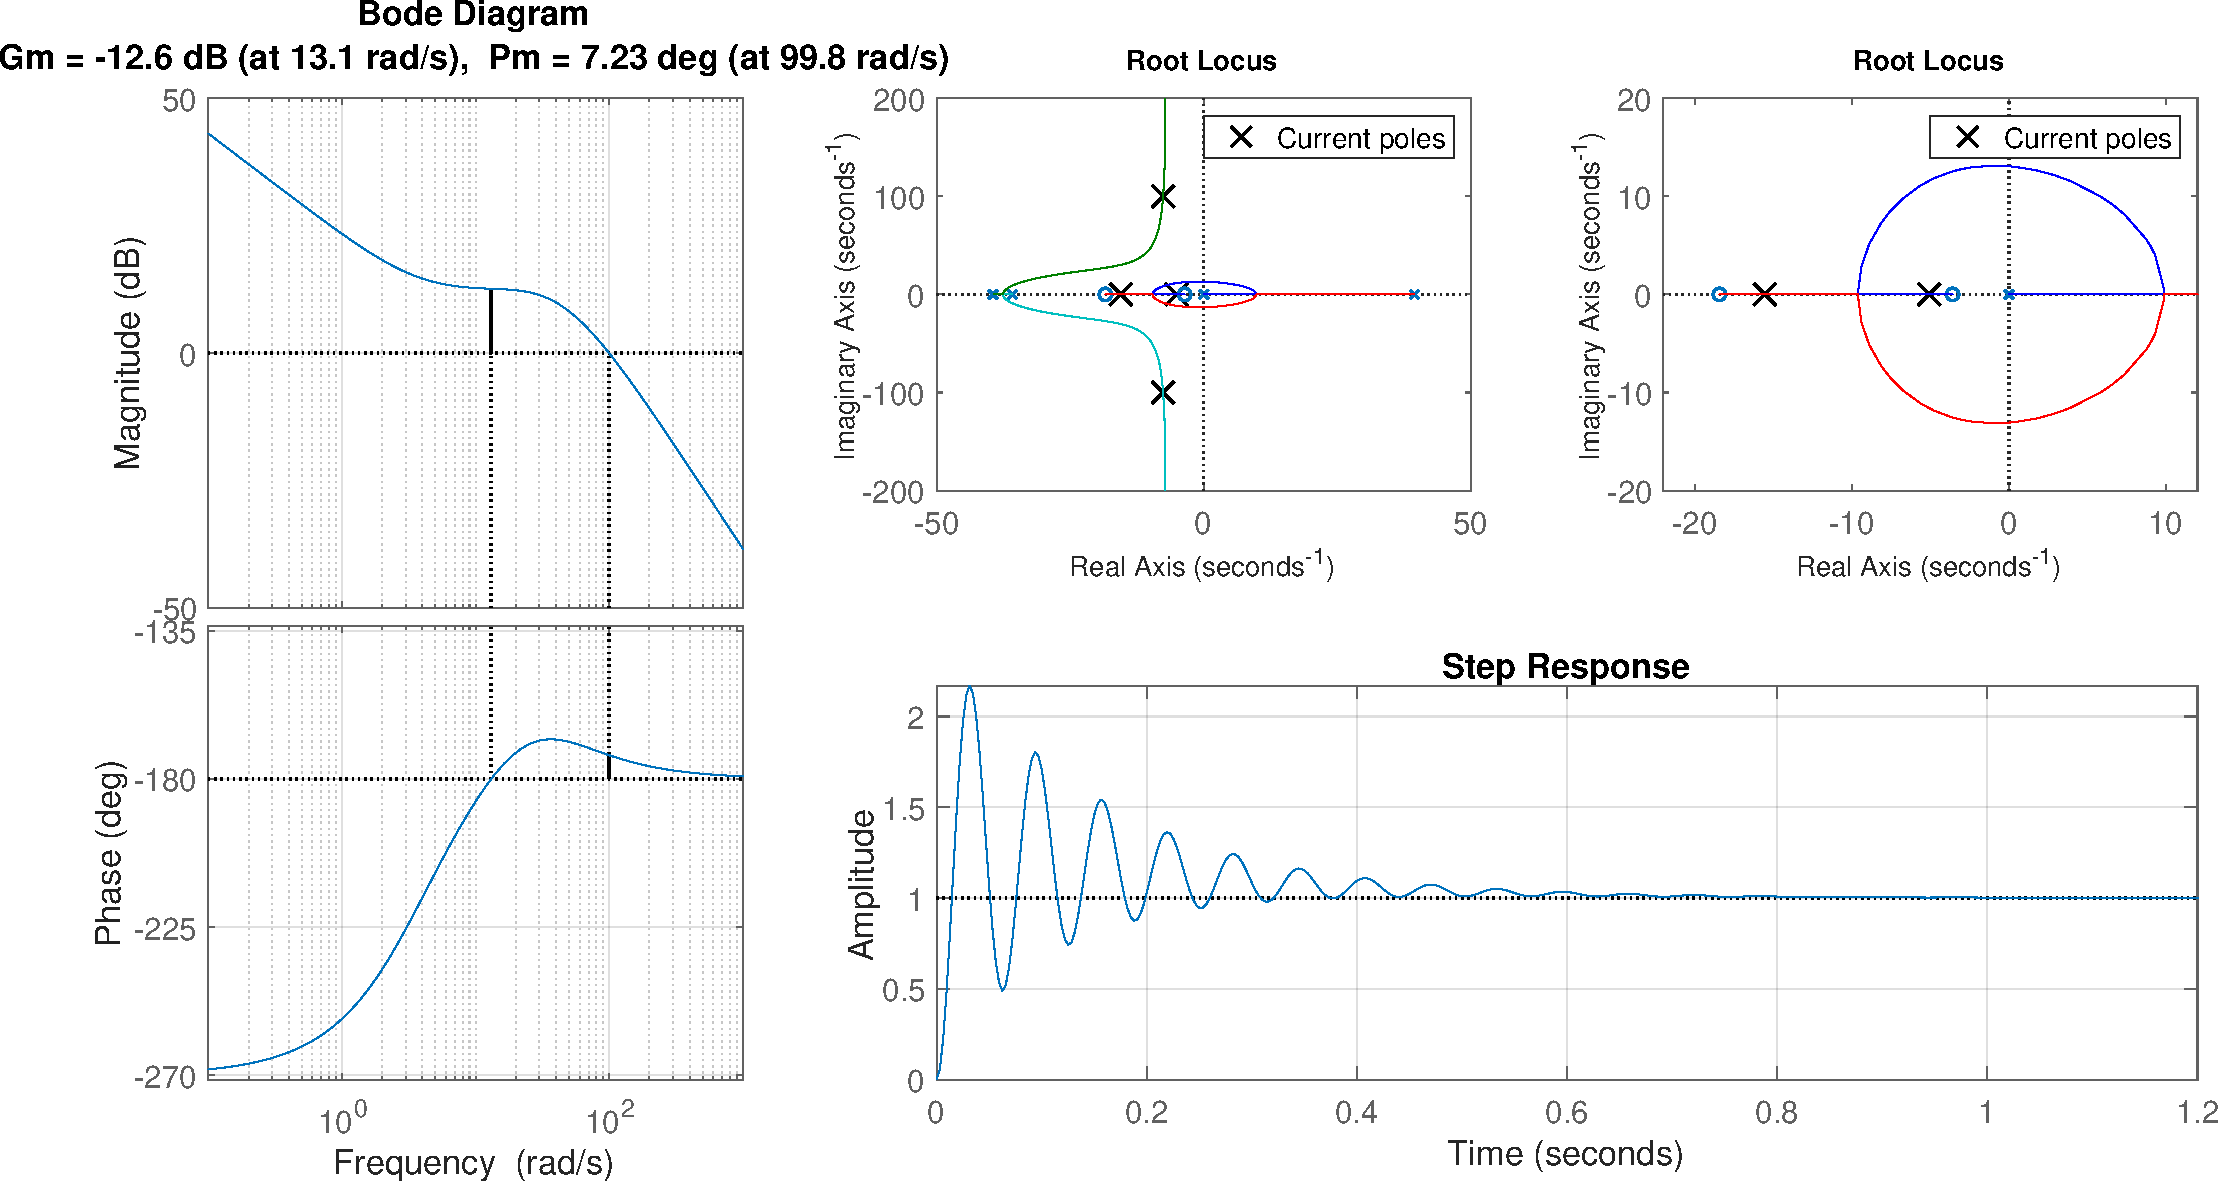
\includegraphics[width=1\linewidth]{./img/MATLAB/controllers/PID_classical.pdf}
    \caption{Bode Plot, Root Locus and Step Response (PID classic)}
    \label{fig:pid_classical_bode}
\end{figure}

Eigenvalues of the system matrix have been computed since eigenvalues with negative real parts indicate stability, as well as a positive phase margin.
Indeed, the resulting system is overall stable.
Nevertheless, the experimental results obtained from the physical tests were not as expected.
A potential explanation could be that the classical PID may introduce some issues due to the integral path and the non-linearity of the system.
We have thus considered two expansions of the classical PID that bring improvements on the control of the system, that are the anti-windup (Section \ref{subsubsec:pid_anti_windup}) and the gain scheduling (Section \ref{subsubsec:pid_gain_scheduling}).



\subsubsection{PID with Anti-Windup correction}
\label{subsubsec:pid_anti_windup}

The Anti-windup variation of the PID is introduced in order to avoid the windup of the integration path when the saturation of the actuator occurs.
The integrator windup occurs when the actuator saturates and the integration part makes the error signal to increase.
This causes the degradation of the rise time of the step response, and possibly leading to higher overshoot.

The basic idea to avoid these issues is to apply a conditional integration.
The controller output is thus compared with the limits, and whenever there is some indication that saturation causes error accumulation, the integrator in PID controller is turned off.

\paragraph{Step Response}

Figure \ref{fig:pid_anti_windup_step_response} shows the response of the system state to a reference step input.
The stability of the dynamics can be observed, specifically considering the most relevant parameters such as the position of the sphere and the current flowing through the coils.
The analytical procedure is the same as for the classical PID, and thus the controller gains that have been used are the ones described in Section \ref{subsubsec:pid_classic}.

\begin{figure}[H]
    \centering
    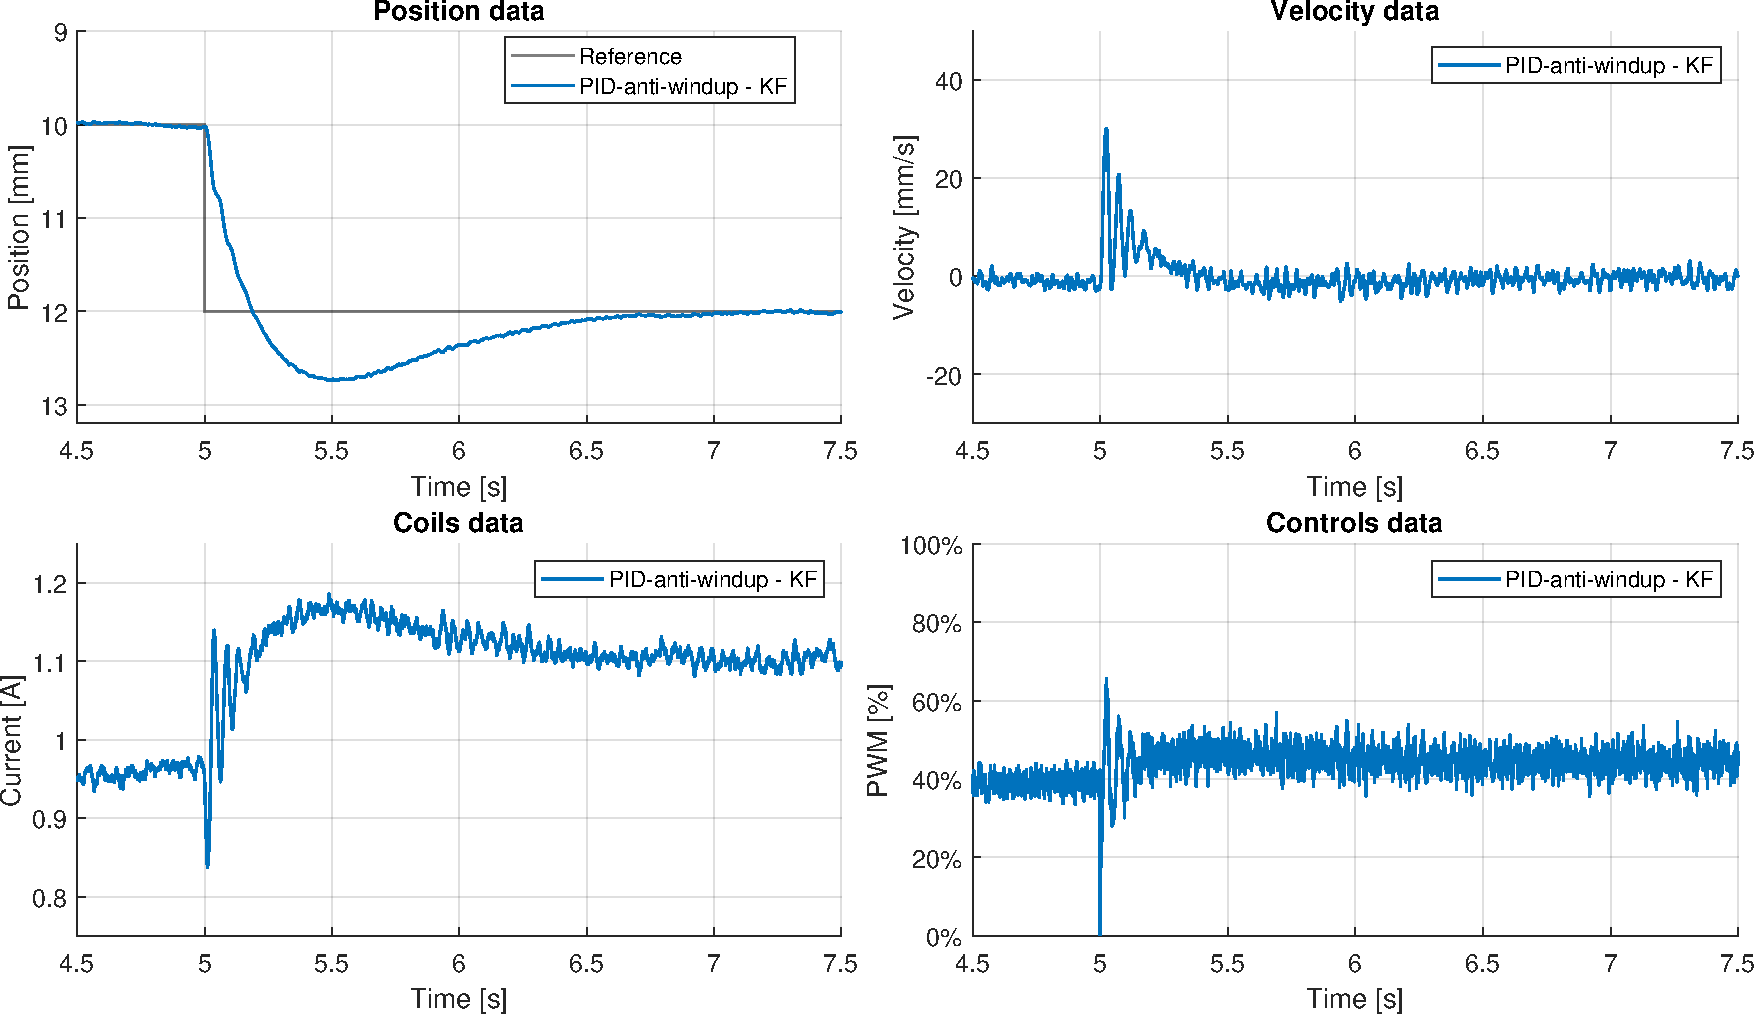
\includegraphics[width=1\linewidth]{./img/MATLAB/results/step_PID_anti_windup_KF.pdf}
    \caption{Step Response (PID anti-windup)}
    \label{fig:pid_anti_windup_step_response}
\end{figure}



\subsubsection{PID with gain scheduling}
\label{subsubsec:pid_gain_scheduling}

Gain scheduling is usually used for highly non-linear systems due to the ease of the implementation and its affordability.
This method tunes PID controllers for a series of steady-state operating points of the plant.

In the considered system, the space interval where the sphere moves has been divided into several points that represent our steady-state operating conditions, and the state-space system has been linearized at each operating condition.
The set of operating conditions has to be large enough in order to get good performance everywhere, as well as the structure and the stability of the model changes when the sphere moves within the range of positions.
As a second step, the controller gains have been tuned for each of these operating points.
The controller develops a set of curves that gradually change the gain parameters from one operating position to another.
In this way the sphere can move within the overall space range.

\paragraph{Bode Diagram}

Several curves describing the system behavior corresponding to each operating point have been plotted in order to discuss the stability conditions.
Table \ref{tab:pid_gain_scheduling_gains} reports the gain parameters for each of the selected operating points.

\begin{table}[H]
    \centering

    \begin{tabular}{|c|c|c|c|}
        \hline
        $z [mm]$ & $K_p$  & $K_i$   & $K_d$   \\
        \hline
        $5$      & $-102$ & $-306$  & $-4.64$ \\
        $8$      & $-136$ & $-408$  & $-6.18$ \\
        $12$     & $-183$ & $-550$  & $-8.34$ \\
        $16$     & $-250$ & $-750$  & $-11.4$ \\
        $20$     & $-342$ & $-1030$ & $-15.5$ \\
        \hline
    \end{tabular}

    \caption{PID controller gains}
    \label{tab:pid_gain_scheduling_gains}

\end{table}

\begin{figure}[H]
    \centering
    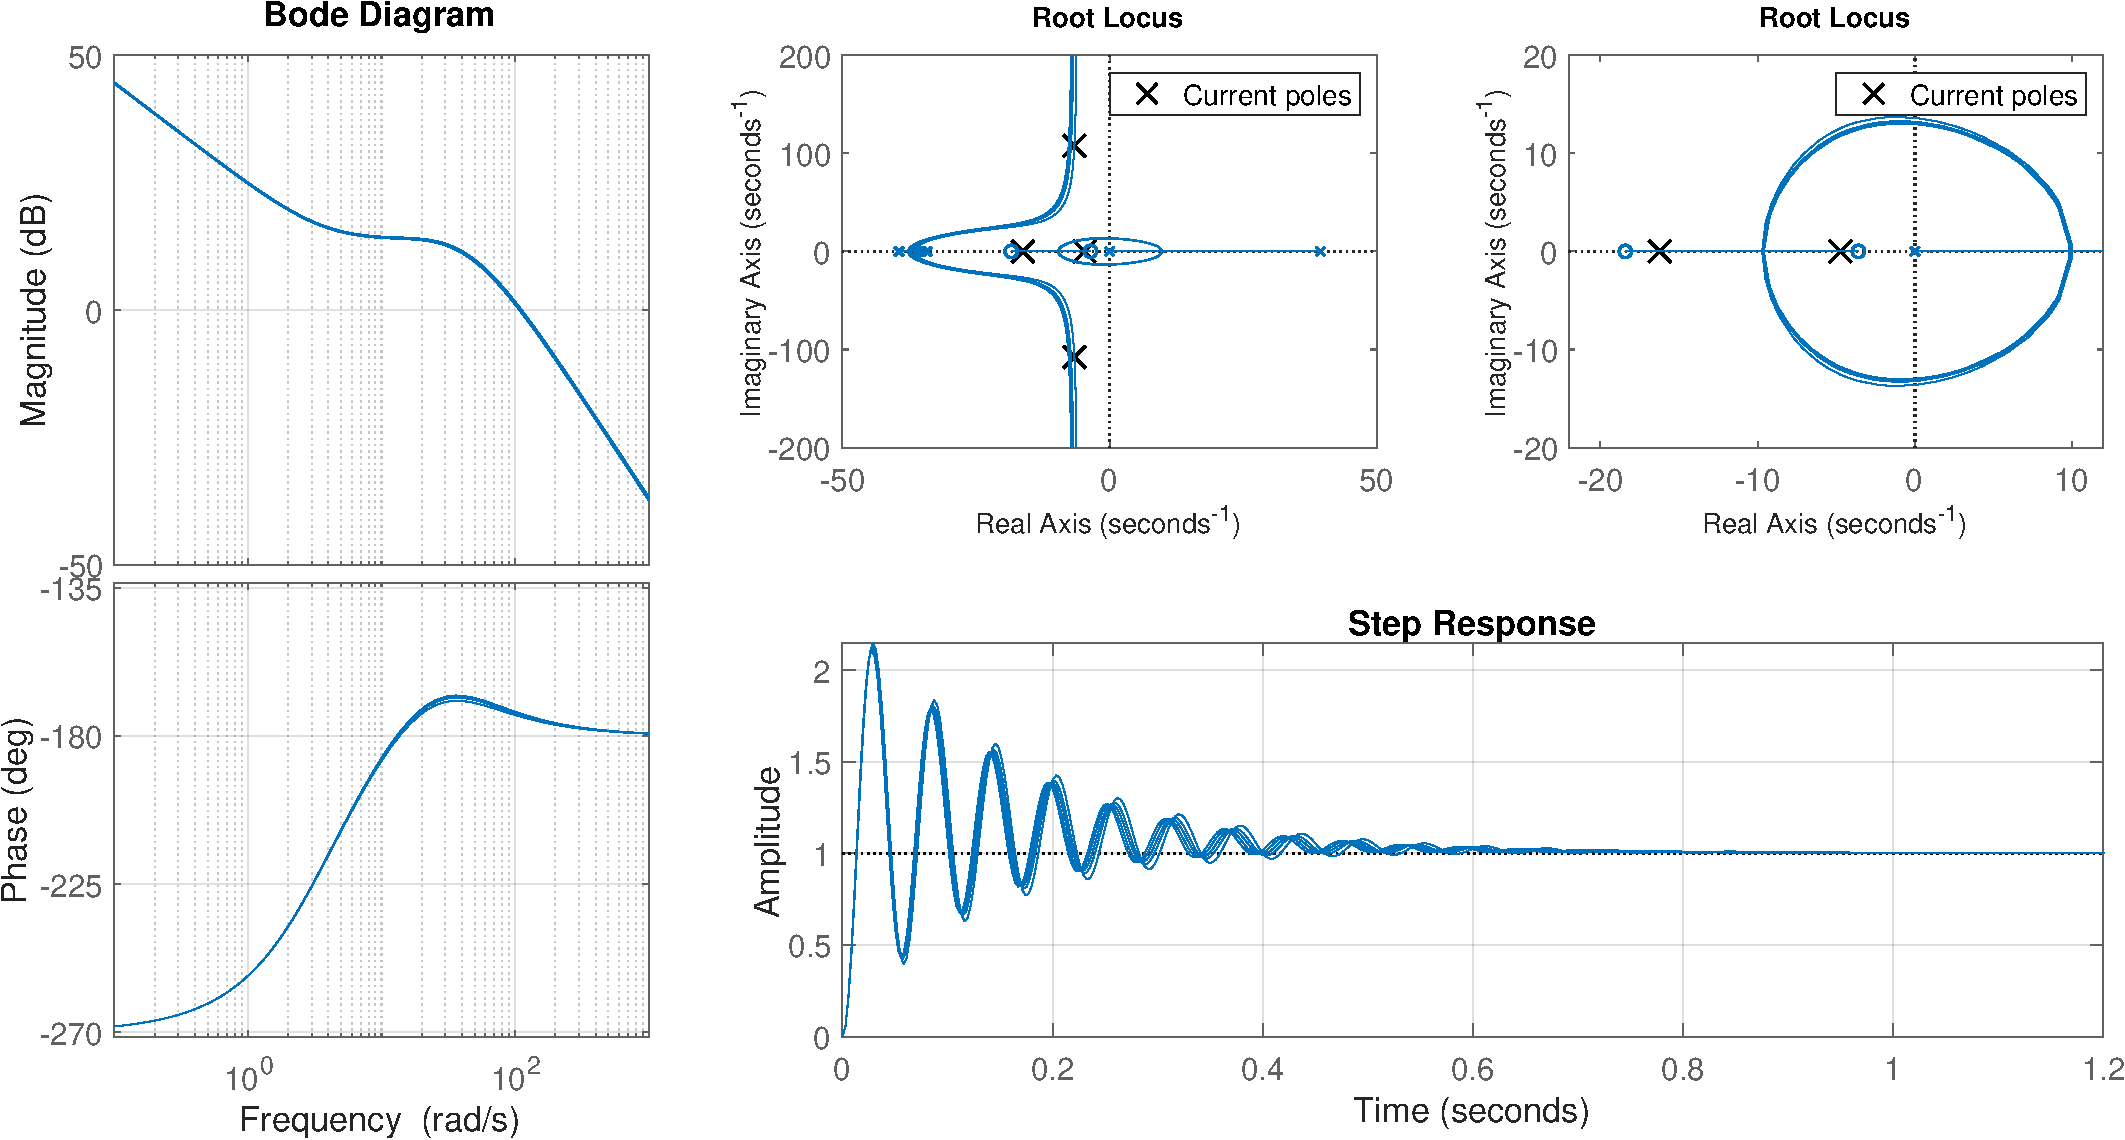
\includegraphics[width=1\linewidth]{./img/MATLAB/controllers/PID_gain_scheduling.pdf}
    \caption{Bode plot, Root Locus and Step Response (PID gain scheduling)}
    \label{fig:pid_gain_scheduling_bode_diagram}
\end{figure}

\paragraph{Step Response}

The efficiency of the response of the system state to a reference step input is described in Figure \ref{fig:pid_gain_scheduling_step_response}.

\begin{figure}[H]
    \centering
    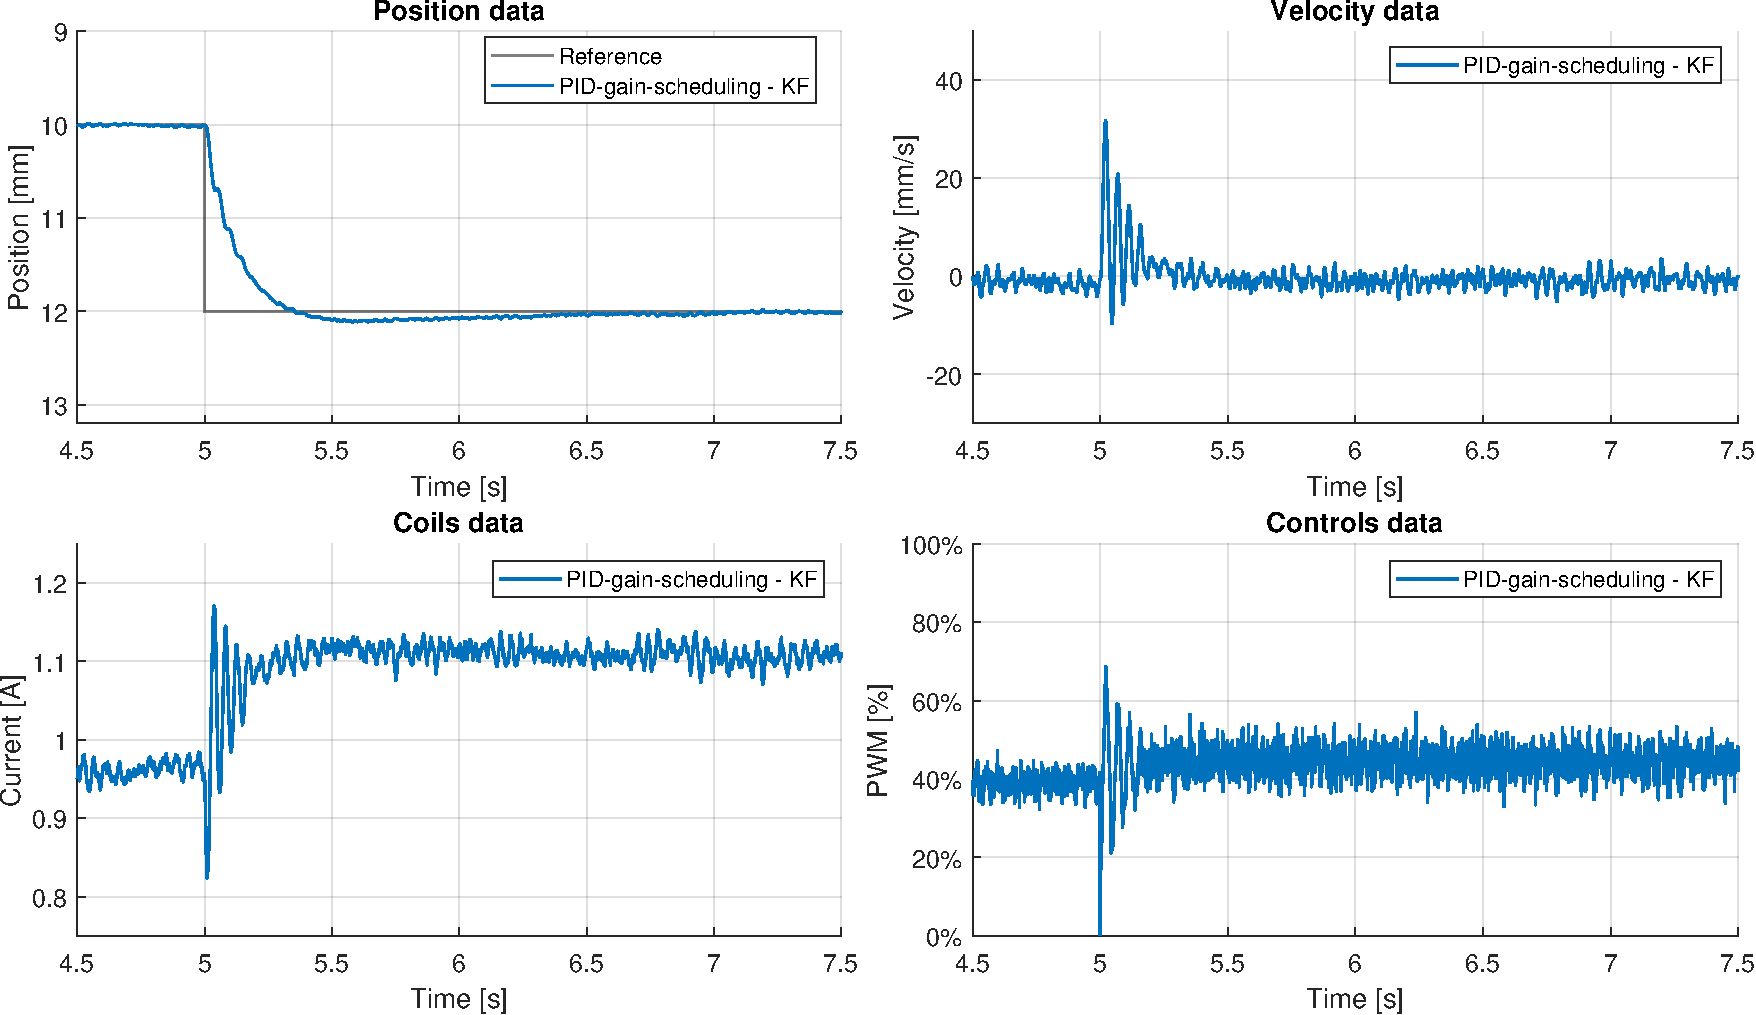
\includegraphics[width=1\linewidth]{./img/MATLAB/results/step_PID_gain_scheduling_KF.pdf}
    \caption{Step Response (PID gain scheduling)}
    \label{fig:pid_gain_scheduling_step_response}
\end{figure}


\subsection{LQ Controllers}
\label{subsec:lq_controllers}

\subsubsection{LQR}
\label{subsubsec:lqr}

\subsubsection{LQR with tracking capabilities}
\label{subsubsec:lqr_tracking}

\subsubsection{LQI}
\label{subsubsec:lqi}
\subsection{MPC Controllers}
\label{subsec:mpc_controllers}

Model Predictive Control (MPC) is an advanced control strategy widely used in industrial and engineering applications. It involves an optimization procedure which is continuously reinitialized as time goes on. This continuous adaptation of the control strategy makes the model very flexible and efficient in various applications.

There exist many versions of MPC but, given the limited computational resources available, we have chosen to implement the linear MPC with constraints on the output variable. This version of MPC is based on a linear model of the system and is computationally less expensive than the nonlinear version.

The system is typically represented in discrete time as:

\begin{equation}
    \begin{aligned}
        \mathbf{x}_{k+1}=\mathbf{A}\mathbf{x}_{k}+\mathbf{B}\mathbf{u}_{k} \\
        \mathbf{y}_{k}=\mathbf{C}\mathbf{x}_{k}
    \end{aligned}
\end{equation}

where $x_k$ is the state vector at time $k$, $\mathbf{u}_k$ is the control input at time $k$, $\mathbf{y}_k$ is the output vector at time $k$, and ($\mathbf{A}$, $\mathbf{B}$, $\mathbf{C}$) are the system matrices.

At eack time step $k$, the MPC controller solves an optimization problem such that the best control strategy is computed over the predefined time horizon, in order to get the state to the desired objective. Once the control action is applied, the system goes forward in time, and the optimization is reinitialized basing on the current state.

The optimization problem typically aims to minimize the objective function reported above, where the trade-off between tracking error and control effort over a finite prediction horizon $N$ is researched:

\begin{equation}
    \mathcal{J} = \sum_{k=0}^{N-1} \left[ (\mathbf{x}_{k+1} - \mathbf{x}_{\text{ref}})^\top \mathbf{Q} (\mathbf{x}_{k+1} - \mathbf{x}_{\text{ref}}) + \mathbf{u}_k^\top \mathbf{R} \mathbf{u}_k \right],
    \label{eq:mpc_objective}
\end{equation}

where $\mathbf{x}_{\text{ref}}$ is the reference trajectory, $\mathbf{Q}$ is the weighting matrix for tracking error, and $\mathbf{R}$ is the weighting matrix for control effort.

At each time step $k$, MPC solves the optimization problem:

\begin{equation}
    \min_{\mathbf{u}_k, \ldots, \mathbf{u}_{k+N-1}} \mathcal{J}
\end{equation}

subject to:

\begin{equation}
    \mathbf{x}_{k+i+1} = \mathbf{A} \mathbf{x}_{k+i} + \mathbf{B} \mathbf{u}_{k+i}, \quad i = 0, \ldots, N-1.
\end{equation}

Only the first control input $\mathbf{u}_k$ is applied to the system, and the process is repeated at the next step. Since the optimization is done continuously and at each time step, the controller is robust so that if the system starts to deviate or the dynamics change over time we can modify the control behavior.

MPC is an attractive approach also because constraints can be imposed on the state or on the input. Indeed, the actuator physically has a saturation limit which cannot be overcome. Another advantage is that this control strategy works for nonlinear systems.

Since the initialization is repeated at each time step, fast hardware are necessaries.

\paragraph{Design} This efficient control strategy has also been implemented. Shorter prediction horizon has been selected to reduce computational effort.

\begin{equation}
    \begin{aligned}
        \textbf{Prediction Horizon} = 0.1s \\ \textbf{Control Horizon}=0.01s
    \end{aligned}
\end{equation}

Constraints on the position and on the control are applied:

\begin{table}[H]
    \centering
    \begin{tabular}{|c|c|c|}
        \hline
        \textbf{Variable} & \textbf{Max} & \textbf{Min} \\ \hline
        Position          & 20 mm        & 0 mm         \\ \hline
        Control           & 1            & 0            \\ \hline
        \hline
    \end{tabular}
    \caption{Constraints for the MPC controller}
\end{table}

\paragraph{Step Response} The system response to an applied step signal is reported in Figure below.

\begin{figure}[H]
    \centering
    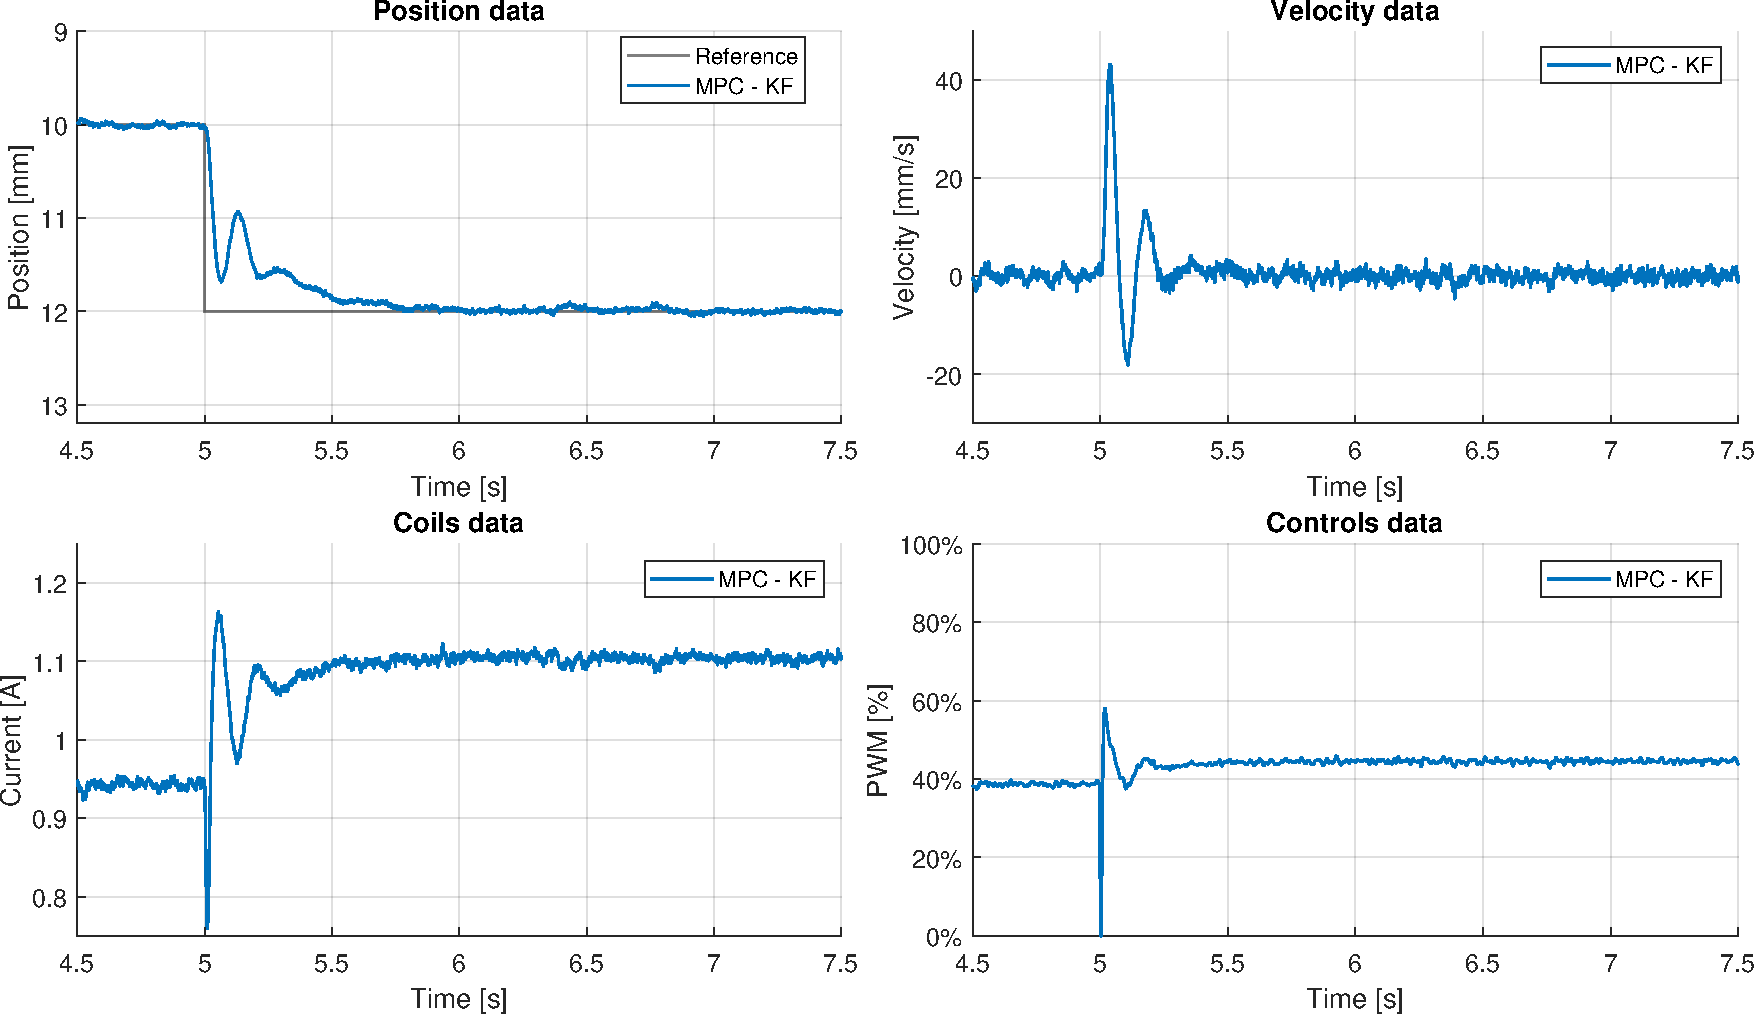
\includegraphics[width=1\linewidth]{./img/MATLAB/results/step_MPC_KF.pdf}
    \caption{Step Response (MPC)}
    \label{fig:step_MPC}
\end{figure}
